\documentclass[../main.tex]{subfiles}
\begin{document}
	
	\section{Lista 6}
	\begin{exercicio}{1}
		(T. Apostol; seção 10.5; exercícios 1, 4 e 9)
		
		Desenhar em ambiente computacional o campo e o caminho. Resolver manualmente e computacionalmente a integral de linha. Escolha 2 (ou mais) pontos da curva para indicar ambos os vetores do integrando: tangente da curva e o campo no ponto específico.
		
		\begin{enumerate}
			\item[1.] $f(x,y)=(x^2-2xy)\textbf{i} + (y^2-2xy)\textbf{j}$, de $(-1,1)$ até $(1,1)$ ao longo da parábola $y=x^2$.
			\item[4.] $f(x,y)=(x^2+y^2)\textbf{i}+(x^2-y^2)\textbf{j}$, de $(0,0)$ até $(2,0)$ ao longo da curva $y=1-|1-x|$.
			\item[9.] $\int_C (x^2-2xy)dx+(y^2-2xy)dy$, onde $C$ é o caminho de $(-2,4)$ até $(1,1)$ ao longo da parábola $y=x^2$.   
		\end{enumerate}
	\end{exercicio}
	\begin{solucao}
		\begin{enumerate}
			\item[1.] Seja $\alpha(t)=(t,t^2)\Rightarrow \alpha'(t)=(1,2t)$, onde $\alpha$ é parametrização da parábola, com $-1<t<1$. Assim, temos que
			\begin{align*}
				\int_C f\, d\alpha
				&=\int_{-1}^1 f(\alpha(t))\cdot \alpha'(t)\, dt\\
				&=\int_{-1}^1 (t^2-2t^3, t^4-2t^3)\cdot (1,2t)\, dt\\
				&=\int_{-1}^1 t^2-2t^3+2t^5-4t^4\, dt \\
				&=\bigg[\frac{t^3}{3}-2\frac{t^4}{4}+2\frac{t^6}{6}-4\frac{t^5}{5}\bigg]\Biggr{|}_{-1}^1\\
				&=\frac{1-(-1)}{3}-\frac{(1-1)}{2}+\frac{1-1}{3}-4\frac{1-(-1)}{5}\\
				&=\frac{2}{3}-\frac{8}{5}\\
				&=-\frac{14}{15}
			\end{align*}
			Abaixo segue o campo e o caminho ilustrados em ambiente computacional, bem como 3 pontos escolhidos da curva, com seus respectivos vetores tangentes e do campo.
			\begin{center}
				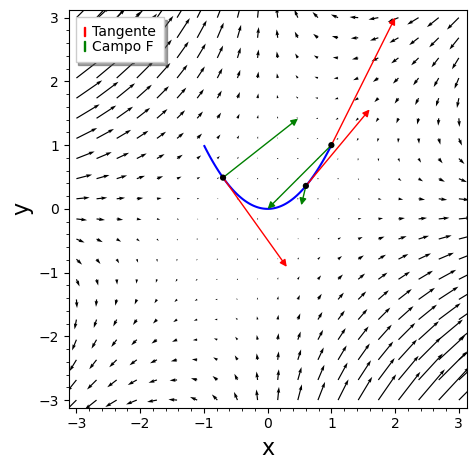
\includegraphics[width=0.25\textwidth]{imagens/lista06/picture_lista06_q01_item01.png}
				\captionof{figure}{Campo vetorial $f$ e caminho $C$}
			\end{center}
			\item[4.] Seja $\alpha(t)=(t,1-|1-t|)$, onde $\alpha$ é parametrização da curva $C$, com $0<t<2$. Devido à função módulo precisamos dividir essa curva $C$ em $C_1$ e $C_2$, de parametrizações $\alpha_1$ e $\alpha_2$ respectivamente, onde
			\[
			\begin{cases} \alpha_1(t)=(t,1-(1-t)), 0<t\leq 1 \\ \alpha_2(t)=(t,1+(1-t)), 1<t<2 \end{cases}\Rightarrow \begin{cases} \alpha_1(t)=(t,t), 0<t\leq 1 \\ \alpha_2(t)=(t,2-t))), 1<t<2 \end{cases}
			\]
			Além disso, note que $\alpha_1'(t)=(1,1)$ e $\alpha_2'(t)=(1,-1)$.
			Assim, temos que
			\begin{align*}
				\int_C f\, d\alpha
				&=\int_{C_1} f\, d\alpha_1+\int_{C_2} f\, d\alpha_2\\
				&=\int_{0}^1 f(\alpha_1(t))\cdot \alpha_1'(t)\, dt+\int_{1}^2 f(\alpha_2(t))\cdot \alpha_2'(t)\, dt\\
				&=\int_{0}^1 (t^2+t^2, t^2-t^2)(1,1)\, dt+\int_{1}^2 (t^2+(2-t)^2, t^2-(2-t)^2)(1,-1)\, dt\\
				&=\int_{0}^1 2t^2\, dt + \int_{1}^2 2(t^2-4t+4)\, dt \\
				&=2\bigg[\frac{t^3}{3}\bigg]\Biggr{|}_{0}^1+2\bigg[\frac{t^3}{3}-4\frac{t^2}{2}+4t\bigg]\Biggr{|}_{1}^2\\				&=\frac{2}{3}+2\bigg(\frac{(8-1)}{3}-2(4-1)+4(2-1)\bigg)\\
				&=\frac{2}{3}+2\frac{1}{3}\\
				&=\frac{4}{3}
			\end{align*}
			
			Abaixo segue o campo e o caminho ilustrados em ambiente computacional, bem como 2 pontos escolhidos da curva, com seus respectivos vetores tangentes e do campo.
			\begin{center}
				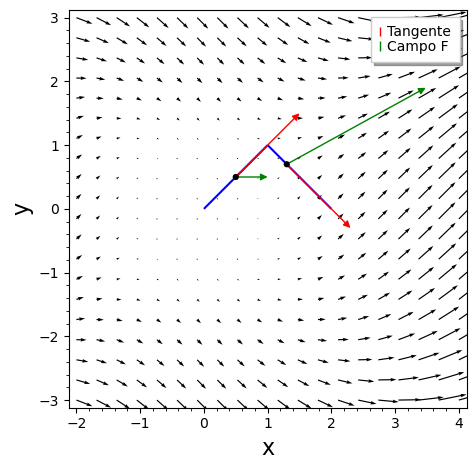
\includegraphics[width=0.25\textwidth]{imagens/lista06/picture_lista06_q01_item04.png}
				\captionof{figure}{Campo vetorial $f$ e caminho $C$}
			\end{center}
			\item[9.] Seja $\alpha(t)=(t,t^2)\Rightarrow \alpha'(t)=(1,2t)$, onde $\alpha$ é parametrização da parábola, com $-2<t<1$. Seja $f(x,y)=(x^2-2xy, y^2-2xy)$. Assim, temos que
			\begin{align*}
				\int_C (x^2-2xy)dx+(y^2-2xy)dy
				&=\int_C f\, d\alpha\\
				&=\int_{-2}^1 f(\alpha(t))\cdot \alpha'(t)\, dt\\
				&=\int_{-2}^1 (t^2-2t^3, t^4-2t^3)\cdot (1,2t)\, dt\\
				&=\int_{-2}^1 t^2-2t^3+2t^5-4t^4\, dt \\
				&=\bigg[\frac{t^3}{3}-2\frac{t^4}{4}+2\frac{t^6}{6}-4\frac{t^5}{5}\bigg]\Biggr{|}_{-2}^1\\
				&=\frac{1+2^3}{3}-\frac{(1-2^4)}{2}+\frac{1-2^6}{3}-4\frac{(1+2^5)}{5}\\
				&=\frac{-180+75-264}{10}\\
				&=-\frac{369}{10}
			\end{align*}
			Abaixo segue o campo e o caminho ilustrados em ambiente computacional, bem como 3 pontos escolhidos da curva, com seus respectivos vetores tangentes e do campo.
			\begin{center}
				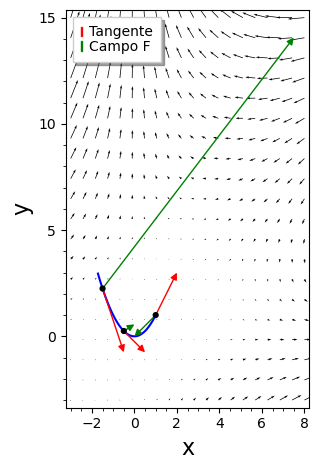
\includegraphics[width=0.25\textwidth]{imagens/lista06/picture_lista06_q01_item09.png}
				\captionof{figure}{Campo vetorial $f$ e caminho $C$}
			\end{center}
		\end{enumerate}
	\end{solucao}
	
	\begin{exercicio}{2}
		(T. Apostol; seção 10.9; exercícios 2 e 8)
		
		\begin{enumerate}
			\item[2.] Encontre a quantidade de trabalho feito pela força $f(x,y)=(x^2-y^2)\textbf{i}+2xy\textbf{j}$ ao mover a partícula (no sentido anti-horário) uma vez ao redor do quadrado limitado pelos eixos de coordenadas e pelas linhas $x=a$ e $y=a$, $a>0$.
			\item[8.] Calcule a integral com respeito ao comprimento de arco $\int_C y^2 ds$, onde $C$ tem a equação vetorial
			\[
			\alpha(t)=a(t-\sin(t))\textbf{i} + a(1-\cos(t))\textbf{j}, 0\leq t\leq 2\pi
			\]
		\end{enumerate}
	\end{exercicio}
	\begin{solucao}
		\begin{enumerate}
			\item[2.] O quadrado limitado pelos eixos de coordenadas e pelas linhas $x=a$ e $y=a$, com $a>0$, no sentido anti-horário, pode ser representado pelas seguintes funções, todas com $t\in(0,a)$:
			\[
			\begin{cases} \alpha_1(t)=(a,t) \\ \alpha_2(t)=(a-t,a)\\ \alpha_3(t)=(0,a-t)\\\alpha_4(t)=(t,0) \end{cases} \Rightarrow \begin{cases} \alpha_1(t)=(0,1) \\ \alpha_2(t)=(-1,0)\\ \alpha_3(t)=(0,-1)\\\alpha_4(t)=(1,0) \end{cases}
			\]
			
			Com isso, podemos calcular o trabalho $W$ como a soma das integrais de linha dessas curvas.
			
			\begin{align*}
				W
				&= \int_0^a (a^2-t^2,2at)(0,1)\, dt + \int_0^a ((a-t)^2-a^2, 2(a-t)a)(-1,0)\, dt \\
				&+ \int_0^a (-(a-t)^2,0)(0,-1)\, dt + \int_0^a (t^2,0)(1,0)\, dt \\
				&= 2a\int_0^a t\, dt - \int_0^a t^2-2at\, dt +\int_0^a t^2\, dt \\
				&= 2a\int_0^a t\, dt - \int_0^a t^2\, dt +2a\int_0^a t\, dt +\int_0^a t^2\, dt \\
				&= 4a \int_0^a t\, dt = 4a\cdot \frac{a^2}{2}\\
				&= 2a^3
			\end{align*}
			
			\item[8.] Note que,
			\begin{align*}
			&\alpha(t)=a\cdot \big(t-\sin(t),1-\cos(t)\big)\\
			&\Rightarrow \alpha'(t)=a\cdot \big(1-\cos(t),\sin(t)\big)\\
			&\Rightarrow \|\alpha'(t)\|=a\cdot \sqrt{1-2\cos(t)+\cos^2(t)+\sin^2(t)}\\
			&\Rightarrow \|\alpha'(t)\|=a\sqrt{2}\sqrt{1-\cos(t)}
			\end{align*}
			Pela definição de integral de linha com respeito ao comprimento de arco, e sendo $f(x,y)=y^2$, temos
			
			\begin{align*}
				\int_C f ds
				&= \int_0^{2\pi} f[\alpha(t)]\|\alpha'(t)\|\, dt\\
				&= \int_0^{2\pi} a^2(1-\cos(t))^2\cdot a\sqrt{2}\cdot \sqrt{1-\cos(t)}\, dt\\
				&= a^3\sqrt{2}\int_0^{2\pi}(1-\cos(t))^{5/2}\, dt\\
				&= 2a^3\sqrt{2}\int_0^{\pi}(1-\cos(2u))^{5/2}\, du\\
				&= 2a^3\sqrt{2}\int_0^{\pi}(1-(1-2\sin^2(u)))^{5/2}\, du\\
				&= 2a^3\sqrt{2}\cdot 4\sqrt{2}\int_0^{\pi}\sin^5(u)\, du\\
				&= 16a^3\int_0^{\pi}(1-\cos^2(u))^2\sin(u)\, du\\
				&= -16a^3\int_1^{-1}(1-v^2)^2\, dv\\
				&= 16a^3\int_{-1}^{1}1-2v^2+v^4\, dv\\
				&= 16a^3\bigg[v-\frac{2v^3}{3}+\frac{v^5}{5}\bigg]\Biggr{|}_{-1}^1=16a^3\bigg(2-\frac{4}{3}+\frac{2}{5}\bigg)\\
				&= \frac{(30-20+6)16a^3}{15}=\frac{256a^3}{15}
			\end{align*}
		\end{enumerate}
	\end{solucao}
	
	\begin{exercicio}{3}
		(T. Apostol; seção 10.13; exercício 6)
		
		Um campo de força $f$ é definido no $\mathbb{R}^3$ pela equação
		\[
		f(x,y,z)=y\textbf{i} + z\textbf{j} +yz\textbf{k}
		\]
		\begin{enumerate}[label=\alph*)]
			\item Determine se $f$ é conservativa ou não.
			\item Calcule o trabalho feito ao mover a partícula pela curva descrita por
			\[
			\alpha(t)=\cos(t)\textbf{i}+\sin(t)\textbf{j}+e^t\textbf{k}
			\]
			Quando $t$ varia de $0$ até $\pi$.
		\end{enumerate}
	\end{exercicio}
	\begin{solucao}
		\begin{enumerate}[label=\alph*)]
			\item Note que
			\[
			\begin{cases} \frac{\partial f_y}{\partial x}=\frac{\partial z}{\partial x}=0\\ \frac{\partial f_x}{\partial y}=\frac{\partial y}{\partial y}=1\end{cases}\Rightarrow  \frac{\partial f_y}{\partial x} \neq \frac{\partial f_x}{\partial y}
			\]
			Logo, $f$ não cumpre as condições necessárias para ser um gradiente e, assim, também não é conservativa.
			\item Para encontrar o trabalho $W$, basta calcular a integral de linha de $f$ ao longo da curva. Sabendo que $\alpha(t)=(\cos(t),\sin(t),e^t)\Rightarrow\alpha'(t)=(-\sin(t), \cos(t), e^t))$
			\begin{align*}
				W
				&= \int_0^\pi f[\alpha(t)]\cdot \alpha'(t)\, dt\\
				&= \int_0^\pi (\sin(t), e^t, e^t\sin(t))(-\sin(t), \cos(t), e^t)\, dt\\
				&= \int_0^\pi -\sin^2t +e^t\cos(t) +e^{2t}\sin(t)\, dt\\
				&= -\int_0^\pi \sin^2t\, dt +\int_0^\pi e^t\cos(t)\, dt +\int_0^\pi e^{2t}\sin(t)\, dt
			\end{align*}
			Vamos calcular cada integral de forma separada.
			\begin{align*}
				\int \sin^2t\, dt
				&= \int \frac{\cos(2t)-1}{2}\, dt\\
				&= \frac{1}{2\cdot 2}\int \cos(u)-1\, du\\
				&= \frac{\sin(u)-u}{4}=\frac{\sin(2t)-2t}{4} 
			\end{align*}
			\begin{align*}
				\int e^t\cos(t)\, dt
				&= e^t\cos(t) +\int e^t\sin(t)\, dt\\
				&= e^t\cos(t) +\bigg(e^t\sin(t)-\int e^t\cos(t)\, dt\bigg)\\
				&\Rightarrow \int e^t \cos(t)\, dt= \frac{e^t}{2}(\cos(t)+\sin(t))
			\end{align*}
			\begin{align*}
				\int e^{2t}\sin(t)\, dt
				&= \frac{e^{2t}}{2}\sin(t)-\frac{1}{2}\int e^{2t}\cos(t)\, dt\\
				&= \frac{e^{2t}}{2}\sin(t)-\frac{1}{2}\bigg(\frac{e^{2t}}{2}\cos(t)+\frac{1}{2}\int e^{2t}\sin(t)\, dt\bigg)\\
				&\Rightarrow \int e^{2t}\sin(t)\, dt+\frac{1}{4}\int e^{2t}\sin(t)\, dt =\frac{e^{2t}}{2}\sin(t)-\frac{e^{2t}}{4}\cos(t)\\
				&\Rightarrow \int e^{2t}\sin(t)\, dt =\frac{e^{2t}}{5}(2\sin(t)-\cos(t))
			\end{align*}
			Agora, avaliando de $0$ a $\pi$, encontramos o trabalho.
			\begin{align*}
				W
				&= -\int_0^\pi \sin^2t\, dt +\int_0^\pi e^t\cos(t)\, dt +\int_0^\pi e^{2t}\sin(t)\, dt\\
				&= \bigg[-\frac{\sin(2t)-2t}{4} + \frac{e^t}{2}(\cos(t)+\sin(t))+\frac{e^{2t}}{5}(2\sin(t)-\cos(t))\bigg]\Biggr{|}_0^\pi\\
				&=-\frac{\sin(2\pi)-2\pi}{4} + \frac{e^\pi}{2}(\cos(\pi)+\sin(\pi))-\frac{e^0}{2}(\cos(0)+\sin(0))\\&+\frac{e^{2\pi}}{5}(2\sin(\pi)-\cos(\pi))-\frac{e^0}{5}(2\sin(0)-\cos(0))\\
				&=\frac{\pi}{2} - \frac{e^\pi}{2}-\frac{1}{2}+\frac{e^{2\pi}}{5}+\frac{1}{5}=\frac{1}{10}(5\pi-5e^\pi-5+2e^{2\pi}+2)
			\end{align*}
			
			Logo, o trabalho é $W = \frac{1}{10}(5\pi-5e^\pi+2e^{2\pi}-3)$
		\end{enumerate}
	\end{solucao}
	
	\begin{exercicio}{4}
		(T. Apostol; seção 10.18; exercícios 3 e 9)
		
		Determine se $f$ é gradiente de um campo escalar ou não. Quando $f$ é gradiente, encontre uma função potencial correspondente $\varphi$.
		\begin{enumerate} 
			\item[3.] $f(x,y)=(2xe^y+y)\textbf{i}+(x^2e^y+x-2y)\textbf{j}$.
			\item[9.] $f(x,y,z)=3y^4z^2\textbf{i}+4x^3z^2\textbf{j}-3x^2y^2\textbf{k}$
		\end{enumerate}
	\end{exercicio}
	\begin{solucao}
		Se $f=(f_1,\dots,f_n)$ é gradiente de um campo escalar, temos, para uma função potencial $\varphi$, as seguintes igualdades:
		\[
		\begin{cases}
			\frac{\partial \varphi}{\partial e_1}=f_1\\
			\dots\\
			\frac{\partial \varphi}{\partial e_n}=f_n
		\end{cases}
		\Rightarrow
		\begin{cases}
			\varphi = \int f_1(x_1,\dots, x_n)\, de_1+A_1(x_2, \dots,x_n)\\
			\dots\\
			\varphi = \int f_n(x_1,\dots, x_n)\, de_n+A_n(x_1,\dots, x_{n-1})
		\end{cases}
		\]
		Utilizando essa lógica, podemos tentar encontrar a função potencial correspondente às questões 3 e 9.
		\begin{enumerate}
			\item[3.] Encontrando as integrais indefinidas, temos que, com relação $x$,
			\begin{align*}
				\varphi
				&=\int (2xe^y+y) \, dx+A_1(y)\\
				&= 2e^y\int x \, dx+y\int\, dx + A_1(y)\\
				&= x^2e^y + xy + A_1(y)
			\end{align*}
			Já com relação a $y$,
			\begin{align*}
				\varphi
				&= \int (x^2e^y+x-2y) \, dy + A_2(x)\\
				&= x^2\int e^y \, dy + x\int \, dy -2\int y \, dy + A_2(x)\\
				&= x^2e^y + xy - y^2 + A_2(x) 
			\end{align*}
			
			Assim, temos que
			\[
			x^2e^y + xy + A_1(y)=x^2e^y+xy-y^2+A_2(x)\Rightarrow \begin{cases}
				A_1(y)=-y^2\\
				A_2(x)=0
			\end{cases}
			\]
			Portanto, $f$ é gradiente de um campo escalar, e sua função potencial correspondente é $\varphi=x^2e^y+xy-y^2$.
			\item[9.] Encontrando as integrais definidas, temos que, com relação a $x$,
			\[
			\varphi=\int (3y^4z^2) \, dx + A_1(y,z)=3xy^4z^2+A_1(y,z)
			\]
			Já com relação a $y$,
			\[
			\varphi= \int (4x^3z^2) \, dy + A_2(x,z)=4x^3yz^2 +A_2(x,z)
			\]
			Já com relação a $z$,
			\[
			\varphi= \int (-3x^2y^2)\, dz + A_3(x,y)=-3x^2y^2z+A_3(x,y)
			\]
			Note que, neste caso, não existe uma função $\varphi$ que cumpra essas três igualdades, o que significa que $f$ não é gradiente de um campo escalar.
		\end{enumerate}
	\end{solucao}
\end{document}